\documentclass{article}
\usepackage{graphicx}
\usepackage{amsmath}
\usepackage{pgfplots}
\pgfplotsset{compat=1.16}
\usepackage{hyperref}
\usepackage{textcomp}

\title{Performance Comparison of Matrix Multiplication in Python, Java, and C}
\author{Jakub Jazdzyk}
\date{\today}

\begin{document}

\maketitle

\section{Introduction}

In this assignment, I compare the performance of a basic matrix multiplication algorithm implemented in three programming languages: Python, Java, and C. The goal is to analyze the efficiency of each language when handling matrix multiplication, considering factors such as execution time, memory usage, and computational overhead.

\section{Methodology}

The matrix multiplication algorithm was implemented using the standard \(O(n^3)\) complexity method. The algorithms were tested with increasingly larger matrix sizes to observe performance scalability.

The experiments involved measuring:

\begin{itemize}
    \item Execution time (in seconds)
    \item Memory usage during execution (in MB)
    \item CPU usage
\end{itemize}

Each language's performance was benchmarked to evaluate speed and resource efficiency, identify bottlenecks, and analyze how the algorithms scale with larger datasets.

\section{Results}

The tables below summarize the execution time, memory usage, and CPU utilization for each language tested with matrix sizes of 10, 80, 200, and 800.

\subsection{Execution Time}

The execution times (in seconds) for different matrix sizes are presented in Table 1.

\begin{table}[h!]
    \centering
    \begin{tabular}{|c|c|c|c|}
    \hline
    Matrix Size & Python (s) & Java (s) & C (s) \\
    \hline
    10  & 0.000278 & 0.017000 & 0.000016 \\
    80  & 0.204845 & 0.010000 & 0.001318 \\
    200 & 2.024001 & 0.037000 & 0.016683 \\
    800 & 35.108645 & 3.868000 & 0.964798 \\
    \hline
    \end{tabular}
    \caption{Execution times for matrix multiplication.}
    \label{tab:execution_time}
\end{table}

\subsection{Memory Usage}

Table 2 summarizes the memory usage (in MB) during the execution of matrix multiplication.

\begin{table}[h!]
    \centering
    \begin{tabular}{|c|c|c|c|}
    \hline
    Matrix Size & Python (MB) & Java (MB) & C (MB) \\
    \hline
    10  & 0.0  & 0.64 & 6.216 \\
    80  & 14.5 & 0.00 & 6.216 \\
    200 & 89.5 & 1.00 & 6.216 \\
    800 & 470.5 & 8.64 & 16.748 \\
    \hline
    \end{tabular}
    \caption{Memory usage during matrix multiplication.}
    \label{tab:memory_usage}
\end{table}

\subsection{CPU Usage}

The CPU usage during execution is summarized in Table 3.

\begin{table}[h!]
    \centering
    \begin{tabular}{|c|c|c|c|}
    \hline
    Matrix Size & Python (\%) & Java (\%) & C (\%) \\
    \hline
    10  & 0.0  & \text{Infinity} & 0.00 \\
    80  & 22.3 & 93.25 & 35.25 \\
    200 & 56.7 & 90.50 & 207.59 \\
    800 & 78.9 & 99.62 & 211.84 \\
    \hline
    \end{tabular}
    \caption{CPU usage during matrix multiplication.}
    \label{tab:cpu_usage}
\end{table}

\section{Analysis of Results}

The results clearly demonstrate the performance differences among the three programming languages.

1. Execution Time: C exhibited the fastest execution times across all matrix sizes, with the most significant performance gap observed in larger matrices. For instance, at a size of 800, C completed the multiplication in approximately 0.964 seconds, while Python took over 35 seconds and Java about 3.87 seconds. This difference highlights the efficiency of C's compiled nature and lower-level memory management.

2. Memory Usage: The memory consumption results indicate that C is the most efficient language. For a matrix size of 800, Python used approximately 470.5 MB of memory, while C only required about 16.748 MB. This suggests that C's memory management is more optimized compared to Python and Java, resulting in lower overhead during execution.

3. CPU Usage: The CPU utilization results reveal interesting insights. Python's CPU usage was considerably lower than that of C and Java, especially for smaller matrices. This can be attributed to Python's higher-level abstractions and interpreted execution, which may not leverage the CPU as effectively. In contrast, C and Java showed higher utilization percentages, indicating that they effectively engage the CPU resources during execution.

\section{Conclusion}

From this assignment, it is clear that C consistently outperforms both Python and Java in terms of execution time, memory usage, and CPU efficiency. While each language has its strengths—Python's simplicity and ease of use, and Java's platform independence—the benchmarks underscore the importance of language choice in performance-critical applications, particularly in scenarios involving large datasets.

To improve the performance of Python and Java implementations, one could explore language-specific optimizations such as parallel processing or utilizing efficient libraries (e.g., NumPy for Python).

The full source code and test results can be found in my GitHub repository: \href{https://github.com/kubajaz/BIG_DATA_INDIVIDUAL_TASKS_JAKUB_JAZDZYK}{GitHub repository}.

The visual representations of the performance metrics can be found below.

\begin{figure}[h!]
    \centering
    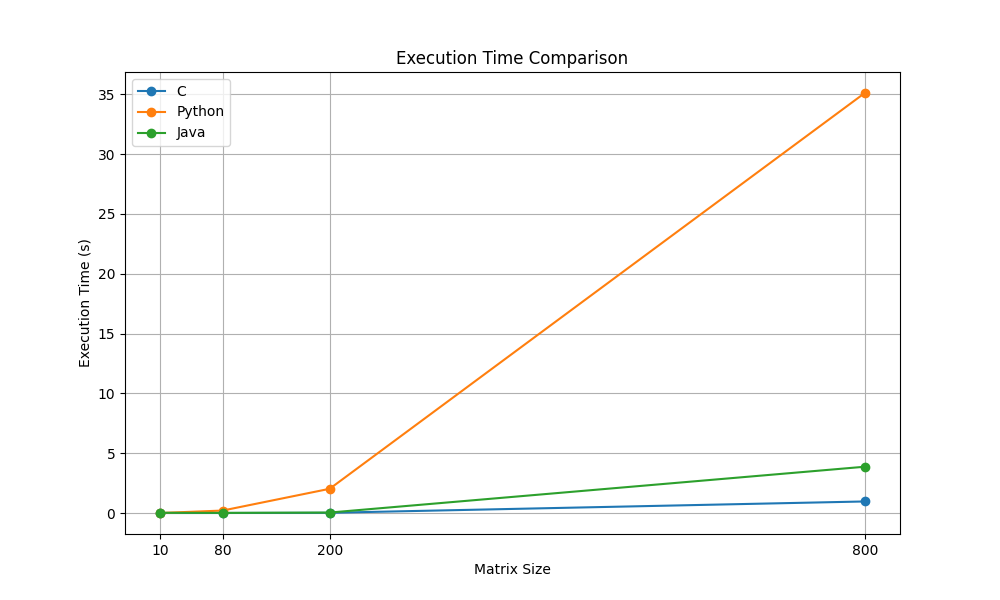
\includegraphics[width=0.8\textwidth]{execution_time_comparison.png}
    \caption{Execution Time vs Matrix Size for Python, Java, and C.}
    \label{fig:execution_time_plot}
\end{figure}

\begin{figure}[h!]
    \centering
    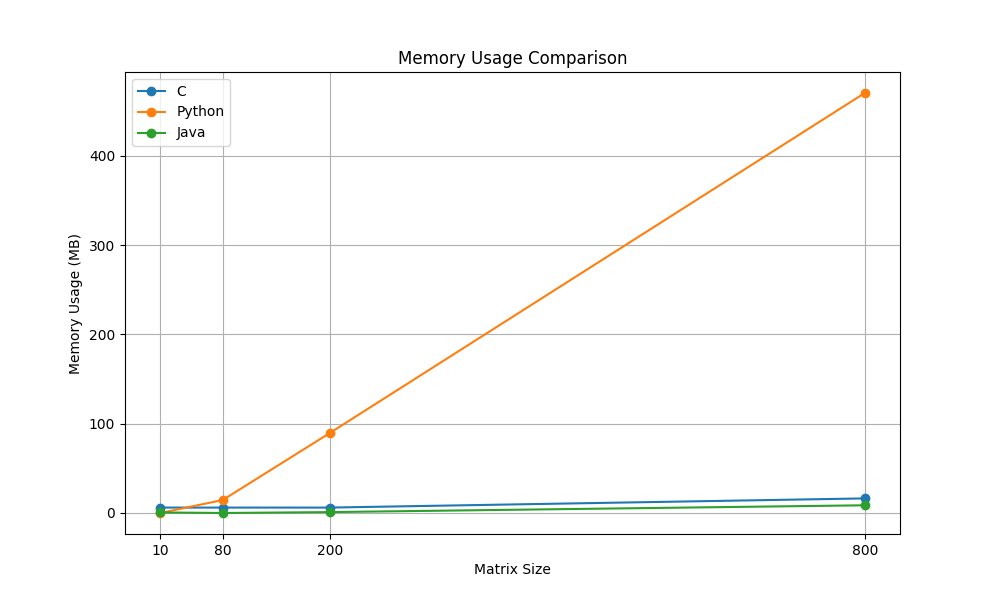
\includegraphics[width=0.8\textwidth]{memory_usage_comparison.png}
    \caption{Memory Usage vs Matrix Size for Python, Java, and C.}
    \label{fig:memory_usage_plot}
\end{figure}

\begin{figure}[h!]
    \centering
    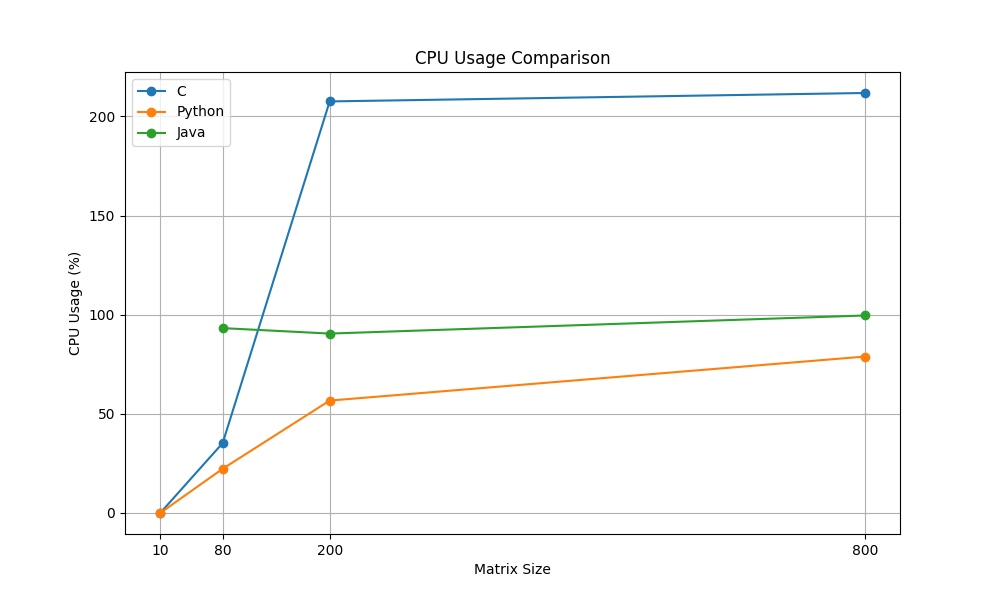
\includegraphics[width=0.8\textwidth]{cpu_usage_comparison.png}
    \caption{CPU Usage vs Matrix Size for Python, Java, and C.}
    \label{fig:cpu_usage_plot}
\end{figure}

\end{document}
